%%% License: Creative Commons Attribution Share Alike 4.0 (see https://creativecommons.org/licenses/by-sa/4.0/)


%%%%%%%%%%%%%%%%%%%%%%%%%%%%%%%%%%%%%%%%%

%----------------------------------------------------------------------------------------
%	PACKAGES AND OTHER DOCUMENT CONFIGURATIONS
%----------------------------------------------------------------------------------------

\documentclass{article}

\usepackage{amssymb}

\usepackage{enumitem}
\usepackage[usenames,dvipsnames]{color}
\usepackage{fancyhdr} % Required for custom headers
\usepackage{lastpage} % Required to determine the last page for the footer
\usepackage{extramarks} % Required for headers and footers
\usepackage[usenames,dvipsnames]{color} % Required for custom colors
\usepackage{graphicx} % Required to insert images
\usepackage{listings} % Required for insertion of code
\usepackage{courier} % Required for the courier font
\usepackage[table]{xcolor}
\usepackage{amsfonts,amsmath,amsthm,parskip,setspace,url}
\usepackage[section]{placeins}
\usepackage[a4paper]{geometry}
\usepackage[USenglish]{babel}
\usepackage[utf8]{inputenc}
\usepackage{hyperref}

%Graphics:
\usepackage{tikz}
\usepackage{tkz-graph}
\usepackage{caption}


% Margins
\topmargin=-0.45in
\evensidemargin=0in
\oddsidemargin=0in
\textwidth=6.5in
\textheight=9.0in
\headsep=0.6in

\linespread{1.1} % Line spacing

%----------------------------------------------------------------------------------------
%	DOCUMENT STRUCTURE COMMANDS
%	Skip this unless you know what you're doing
%----------------------------------------------------------------------------------------

% Header and footer for when a page split occurs within a problem environment
\newcommand{\enterProblemHeader}[1]{
\nobreak\extramarks{#1}{#1 continued on next page\ldots}\nobreak
\nobreak\extramarks{#1 (continued)}{#1 continued on next page\ldots}\nobreak
}

% Header and footer for when a page split occurs between problem environments
\newcommand{\exitProblemHeader}[1]{
\nobreak\extramarks{#1 (continued)}{#1 continued on next page\ldots}\nobreak
\nobreak\extramarks{#1}{}\nobreak
}

\setcounter{secnumdepth}{0} % Removes default section numbers
\newcounter{homeworkProblemCounter} % Creates a counter to keep track of the number of problems

\newcommand{\homeworkProblemName}{}
\newenvironment{ex}[1][Problem \arabic{homeworkProblemCounter}]{ % Makes a new environment called homeworkProblem which takes 1 argument (custom name) but the default is "Problem #"
\stepcounter{homeworkProblemCounter} % Increase counter for number of problems
\renewcommand{\homeworkProblemName}{#1} % Assign \homeworkProblemName the name of the problem
\section{\homeworkProblemName} % Make a section in the document with the custom problem count
\enterProblemHeader{\homeworkProblemName} % Header and footer within the environment
}{
\exitProblemHeader{\homeworkProblemName} % Header and footer after the environment
}

\newcommand{\problemAnswer}[1]{ % Defines the problem answer command with the content as the only argument
\noindent\framebox[\columnwidth][c]{\begin{minipage}{0.98\columnwidth}#1\end{minipage}} % Makes the box around the problem answer and puts the content inside
}

\newcommand{\homeworkSectionName}{}
\newenvironment{homeworkSection}[1]{ % New environment for sections within homework problems, takes 1 argument - the name of the section
\renewcommand{\homeworkSectionName}{#1} % Assign \homeworkSectionName to the name of the section from the environment argument
\subsection{\homeworkSectionName} % Make a subsection with the custom name of the subsection
\enterProblemHeader{\homeworkProblemName\ [\homeworkSectionName]} % Header and footer within the environment
}{
\enterProblemHeader{\homeworkProblemName} % Header and footer after the environment
}

\newif\ifsolutions

%----------------------------------------------------------------------------------------
%----------------------------------------------------------------------------------------
%----------------------------------------------------------------------------------------
% Set up the header and footer
\pagestyle{fancy}
\lhead[c]{\textbf{{\color[rgb]{.5,0,0} K{\o}benhavns\\Universitet }}\\} % Top left header
\chead{\textbf{{\color[rgb]{.5,0,0} \Class }}\\ \hmwkTitle \\ \firstxmark} % Top center head
\rhead{\instructor \\ \theprofessor \\} % Top right header
\lfoot{\lastxmark} % Bottom left footer
\cfoot{} % Bottom center footer
\rfoot{Page\ \thepage\ of\ \protect\pageref{LastPage}} % Bottom right footer
\renewcommand\headrulewidth{0.4pt} % Size of the header rule
\renewcommand\footrulewidth{0.4pt} % Size of the footer rule

\setlength\parindent{12pt} % Removes all indentation from paragraphs







%----------------------------------------------------------------------------------------
%	NAME AND CLASS SECTION
%----------------------------------------------------------------------------------------

\newcommand{\hmwkTitle}{Final Exam} % Assignment title
\newcommand{\Class}{Mechanism Design} % Course/class
\newcommand{\instructor}{Fall 2019} % TA
\newcommand{\theprofessor}{Prof. Egor Starkov} % Professor

%\theoremstyle{definition} \newtheorem{ex}{\textbf{\Large{Exercise & #}\\}}
\setlength{\parskip}{6 pt}




















%%%%%%%%%%%%%%%%%%%%%%%%%%%%%%%%%%%%%%%%%%%%%%%%%%%%%%%%%%%%%%%%%%%%%%%%%%%%%%%%%%%%%%
%\solutionsfalse
\solutionstrue
%%%%%%%%%%%%%%%%%%%%%%%%%%%%%%%%%%%%%%%%%%%%%%%%%%%%%%%%%%%%%%%%%%%%%%%%%%%%%%%%%%%%%%


\begin{document}

\begin{center}
	{\Huge Final Exam
	\ifsolutions (with Solutions) \fi}
\end{center}
\bigskip

\ifsolutions
%The solutions below are meant to explain a possible way to solve the given problems. They are not meant to present an answer that would receive maximal grade for each question, and neither should they be understood as a grading rubric.
\else
Write up your responses to questions below, and submit them to Absalon (one file per group). Show your work and explain your answers. The deadline to submit the responses is Oct 25, 12:00 (noon). Satisfactory performance on this midterm is a prerequisite to participating in the final exam.

Some exercises are open ended in that they may not have a unique correct answer. If you think there is a typo in a problem, please report it to me by midnight on Oct 18 and I will issue a correction if required. If you think there is a typo, and the deadline has passed, attempt to fix it yourself as best you can and proceed with the remainder of the problem. 
\fi


%%-----------------------------------------------------------------------------------------------------

\begin{ex}
	Dynamic Efficient
	
	\ifsolutions
	\subsection*{Solution}
	...
	\fi
\end{ex}



%%-----------------------------------------------------------------------------------------------------

\begin{ex}
	Dynamic Optimal
	
	\ifsolutions
	\subsection*{Solution}
	...
	\fi
\end{ex}



%%-----------------------------------------------------------------------------------------------------

\begin{ex}
	\textbf{(25 pts)}
	Consider the classic marriage (two sided-matching) model, with finite sets of men and women, $M$ and $W$, (possibly unequal cardinality).  Each man $m \in M$ has height $h_m$; each woman $w \in W$ has height $h_w$.  Preferences are as follows:

	\begin{itemize}
		\item agents prefer mates to have height closer to their own;
		\item agents strictly prefer being matched to remaining single.
	\end{itemize}
	
	Formally, the utility that man $m$ and woman $w$ get from being matched to each other is given by $u_m(w) = u_w(m) = -|h_m - h_w|$, and the utility of being
single is arbitrary low.
	
	In particular, consider a market with $3$ men $M = \{m_1,m_2,m_3\}$ with heights $\{h_{m_1}, h_{m_2}, h_{m_3}\} = \{174,177,184\}$ and $2$ women $W = \{w_1,w_2\}$ with heights $\{h_{w_1}, h_{w_2}\} = \{175,180\}$.
	
	\begin{enumerate}
		\item (5pts) Find the outcome of men-proposing deferred acceptance (M-DA) algorithm in this market.
		\item (5pts) Find the outcome of women-proposing deferred acceptance (W-DA) algorithm in this market.
		\item (5pts) Are there any other stable matchings?
		\item (5pts) Suppose now that players' heights are not observable to the designer (but players still know each everyone's heights). Consider a game in which all player must report their heights before the W-DA algorithm is run. Show that the strategy profile where all players truthfully report their heights is not a Bayes-Nash Equilibrium of this game.
		\item (5pts) Given that all players know everyone's heights, is there a mechanism that the designer can use to elicit players' true heights? (No transfers are allowed.) If yes, describe the mechanism fully and verify that it implements the truthful outcome. If not, argue why not.
	\end{enumerate}
	
	\ifsolutions
	\subsection*{Solution}
	\begin{enumerate}
		\item The answers to parts (1) and (2) are the same: under either algorithm the matches are $(m_1, w_1)$ and $(m_2, w_2)$, while $m_3$ remains single. 
		
		\emph{Grading note} for (1) and (2): partial credit possible if student ran some steps of the algorithm correctly but arrived to a wrong answer.
		\item .
		\item Together with the lattice structure of the set of stable matchings and the fact that the outcomes of M-DA and W-DA are always the maximal and minimal elements of this lattice, the fact that the two coincide implies that the set of stable matchings is a singleton (i.e., the outcome identified in (1)-(2) is unique). 
		
		\emph{Grading note}: to get full credit, it is enough to claim uniqueness and mention lattice structure in the explanation. If the student solved (1) and/or (2) incorrectly, arriving to different outcomes in the two questions, then partial credit is available for invoking the lattice structure to say that other stable matchings exist.
		\item If $m_3$ reports his height truthfully then he remains single, while reporting $h_{m_3} = 180$ would lead to him being matched with $w_2$ under W-DA. Man $m_2$ also has a profitable deviation by reporting $h_{m_2} = 175$.
		
		\emph{Grading note}: full credit for identifying one valid profitable deviation.
		\item Ask each player to report \emph{all} players' heights. If all reports coincide, use this heights profile to run M-DA/W-DA algorithm. Otherwise leave everyone unmatched. Truthtelling is an equilibrium of this mechanism: neither of the players matched under truthtelling want to deviate and become unmatched, and $m_3$ is indifferent between reporting truthfully and lying.
		
		\emph{Grading note}: 2 points for asking each player to report all players' heights or some other reporting structure that allows to cross-verify players' reports. 2 more points for specifying the outcome in case of mismatching reports. 
		
		NOTE: another possible correct answer is as follows. Ask each player to report all players' heights. If $4$ out of $5$ reports coincide, use the modal heights profile to run M-DA/W-DA algorithm. Otherwise \emph{match randomly}. Note that random matching is better for $m_3$ than remaining single for sure, so $m_3$ must not be able to invoke this possibility on his own -- hence the 4/5 rule.
	\end{enumerate}
	
	\fi
\end{ex}



%%-----------------------------------------------------------------------------------------------------

\begin{ex}
	\textbf{(25 pts)}
	A consumer is choosing between two Samsung smartphones: the new Galaxy Fold, which costs $p_F = \$ 2000$, and the older Galaxy S10, which costs $p_S = \$1000$. The consumer does not know which of the two is right for her, and she is very afraid of making the wrong choice. 
	
	Formally, from the consumer's point of view, one of the two states is possible: $\omega \in \{F,S\}$. Her expected utility from buying phone $a \in \{F,S\}$ is given by
	\begin{equation*}
		u(a|q) = \mathbb{E}_\omega \left[ v(a,\omega) \mid q \right] - p_a,
	\end{equation*}
	where $q$ denotes the probability that the consumer assigns to state being $\omega = F$, and the state-dependent valuations $v(a,\omega)$ are given by %(in monetary equivalent)
	\begin{center}
		\begin{tabular}{c | c | c |}
			$v(a,\omega)$ 		& $\omega = F$ 	& $\omega = S$ \\ \hline
			$a=F$ (buy Fold)	& $3000$ 	& $0$	\\ \hline
			$a=S$ (buy S10)		& $0$ 	& $1500$	\\ \hline
		\end{tabular}
	\end{center}
	The consumer always has the option (denoted as $a = \varnothing$) to walk away from the purchase, which yields utility zero.
	
	The seller can procure the phones at zero cost, hence his profit $\pi(a)$ is given by
	\begin{equation*}
		\pi(a) = 
		\begin{cases}
			p_F & \text{ if } a=F; \\
			p_S & \text{ if } a=S; \\
			0 & \text{ if } a=\varnothing.
		\end{cases}
	\end{equation*}
	
	\begin{enumerate}
		\item (4pts) Describe the consumer's optimal choice rule $a(q)$ for any given belief $q = \mathbb{P}(\omega=F)$.
		\item (4pts) Write down the consumer's expected utility $U(q) = \max_a u(a|q)$ from following this optimal choice rule $a(q)$. 
		\item (4pts) Write down the company's profit $\Pi(q)$ from the consumer following her optimal choice rule $a(q)$.
	\end{enumerate}

	Suppose that the consumer's prior is $q_0 = \frac{1}{2}$. The seller decides to engage in Bayesian Persuasion: he designs a quiz that, when passed by the consumer, will tell her which phone is likely better for her. Formally, a quiz is an experiment $Q = \left\{ (\tau_1, q_1), (\tau_2, q_2), ... \right\}$, which moves the consumer's belief to $q_k$ with probability $\tau_k$. Naturally, it must be that $\sum_k \tau_k = 1$ and $\sum_k \tau_k q_k = q_0$. Note that posteriors $q_k$ need not be in $\{0,1\}$: the quiz may induce any posterior $q_k \in [0,1]$.
	\begin{enumerate}[resume]
		\item (13pts) Find the quiz/experiment $Q$ that maximizes the seller's expected profit.\\
		\emph{Hint: drawing a graph of $\Pi(q)$ may help you.}
	\end{enumerate}
	
	
	\ifsolutions
	\subsection*{Solution}
	\begin{enumerate}
		\item The consumer's utilities from the three options are given by:
		\begin{align*}
			u(F|q) &= q \cdot 3000 + (1-q) \cdot 0 - 2000 \\
			u(S|q) &= q \cdot 0 + (1-q) \cdot 1500 - 1000 \\
			u(\varnothing|q) &= 0
		\end{align*}
		The three are depicted in Figure \ref{fig:U}.
		Taking the maximum of the three for a given $q$ yields the optimal choice rule
		\begin{equation*}
			a(q) = 
			\begin{cases}
			F & \text{ if } q \geq \frac{2}{3}; \\
			\varnothing & \text{ if } q \in \left[ \frac{1}{3}, \frac{2}{3} \right]; \\
			S & \text{ if } q \leq \frac{1}{3}.
			\end{cases}
		\end{equation*}
		\item From the previous answer, we get
		\begin{equation*}
			U(q) = 1000 \cdot 
			\begin{cases}
			3q - 2 & \text{ if } q \geq \frac{2}{3}; \\
			0 & \text{ if } q \in \left[ \frac{1}{3}, \frac{2}{3} \right]; \\
			0.5 - 1.5q & \text{ if } q \leq \frac{1}{3}.
			\end{cases}
		\end{equation*}
		\item From (1), we have
		\begin{equation*}
			\Pi(q) = 1000 \cdot 
			\begin{cases}
			2 & \text{ if } q \geq \frac{2}{3}; \\
			0 & \text{ if } q \in \left[ \frac{1}{3}, \frac{2}{3} \right]; \\
			1 & \text{ if } q \leq \frac{1}{3}.
			\end{cases}
		\end{equation*}
		\item As suggested by the hint, look at the graph of $\Pi(q)$ depicted in Figure \ref{fig:profit}. %TODO
		The profit $\Pi^*(q)$ that the seller can achieve under the optimal Bayesian Persuasion mechanism is given by the smallest concave envelope of $\Pi(q)$. You can see from the Figure that $\Pi^*(q)$ coincides with $\Pi(q)$ for $q \in NP \equiv \{0\} \cup [2/3,1]$ -- if the consumer's prior belonged to this set then no persuasion mechanism could increase the seller's profit. For any remaining prior (which includes our case, $q_0=1/2$), the optimal persuasion mechanism splits the prior between two closest points in $NP$. In case of prior $q_0 = 1/2$, the optimal persuasion mechanism prescribes posteriors $q_1 = 0$ and $q_2 = 2/3$. The probabilities of these posteriors can then be computed from the consistency requirement (a.k.a. law of total probability):
		\begin{align*}
			\tau_1 \cdot q_1 + \tau_2 \cdot q_2 &= q_0
			\\
			\Leftrightarrow \tau_1 \cdot 0 + \tau_2 \cdot \frac{2}{3} &= \frac{1}{2}
		\end{align*}
		and the requirement $\tau_1 + \tau_2 = 1$. The two together yield $(\tau_1,\tau_2) = (1/4, 3/4)$. Hence the optimal experiment $Q$ induces posterior $q_1 = 0$ with probability $\tau_1 = 1/4$ and posterior $q_2 = 2/3$ with probability $\tau_2 = 3/4$.
		
		\emph{Grading note}: a correct (conditional on parts 1-3) graph of $\Pi^*(q)$ is worth 8 points. Note: graph in Figure \ref{fig:profit_wrong} is \textbf{not} considered correct (since the resulting $\Pi^*(q)$ is not concave).
	\end{enumerate}

	\begin{figure}
		\parbox{0.5\linewidth}{
			\centering
			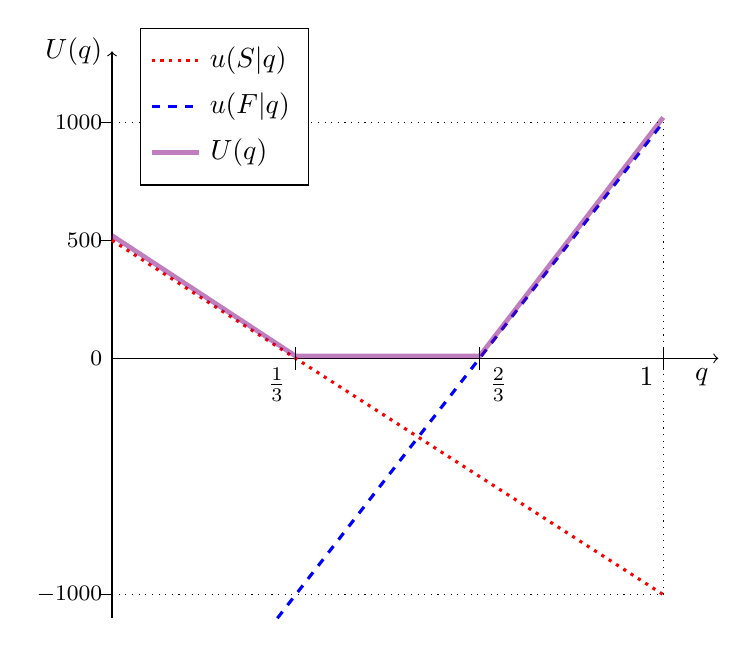
\begin{tikzpicture}[xscale=7,yscale=3]
				\draw[->] (0,0) -- (1.1,0) node[below left]{$q$};
				\draw[->] (0,-1.1) -- (0,1.3) node[left]{$U(q)$};
				\draw (0,0) node[left]{\footnotesize $0$};
				
				% Plot
				\draw[line width=0.4mm, red, dotted] (0,0.5) -- (1,-1);
				\draw[line width=0.4mm, blue, dashed] (0.3,-1.1) -- (1,1);
				\draw[line width=0.6mm, violet, opacity=0.5] (0,0.52) -- (0.333,0.01) -- (0.667,0.01) -- (1,1.02);
				
				% Ticks
				% x axis
				\draw (0.333,0) coordinate(q1) node[below left]{$\frac{1}{3}$};
				\draw (q1) ++(0,-0.05) -- ++(0,0.1);
				
				\draw (0.667,0) coordinate(q2) node[below right]{$\frac{2}{3}$};
				\draw (q2) ++(0,-0.05) -- ++(0,0.1);
				
				\draw (1,0) coordinate(q3) node[below left]{$1$};
				\draw (q3) ++(0,-0.05) -- ++(0,0.1);
				\draw[dotted] (1,-1) -- (1,1);
				
				% y axis
				\draw (0,0.5) coordinate(u1) node[left]{\footnotesize $500$};
				\draw (u1) ++(-0.02,0) -- ++(0.02,0);
				
				\draw (0,1) coordinate(u2) node[left]{\footnotesize $1000$};
				\draw (u2) ++(-0.02,0) -- ++(0.02,0);
				\draw[dotted] (u2) -- ++(1,0);
				
				\draw (0,-1) coordinate(u3) node[left]{\footnotesize $-1000$};
				\draw (u3) ++(-0.02,0) -- ++(0.02,0);
				\draw[dotted] (u3) -- ++(1,0);
				
				%Legend
				\matrix [draw, fill=white, below right] at (0.05,1.4) {
					\draw [line width=0.4mm, red, dotted] ++(-0.3,0) -- ++(0.6,0) node[black,right] {$u(S|q)$}; \\
					\draw [line width=0.4mm, blue, dashed] ++(-0.3,0) -- ++(0.6,0) node[black,right] {$u(F|q)$}; \\
					\draw [line width=0.6mm, violet, opacity=0.5] ++(-0.3,0) -- ++(0.6,0) node[black,right,opacity=1] {$U(q)$}; \\
				};
			\end{tikzpicture}
			\caption{$U(q)$}
			\label{fig:U}
		}
		\parbox{0.5\linewidth}{
			\centering
			\begin{tikzpicture}[xscale=6,yscale=2.5,
					piline/.style={line width=0.4mm, red}
				]
				\draw[->] (0,0) -- (1.1,0) node[below left]{$q$};
				\draw[->] (0,0) -- (0,2.5) node[below left]{$\Pi(q)$};
				\draw (0,0) node[left]{\footnotesize $0$};
				
				% Plot
				% Pi
				\draw[piline] (0,1) -- (0.33,1);
				\draw[red,dotted] (0.33,1) -- (0.33,0);
				\draw[piline] (0.33,0) -- (0.67,0);
				\draw[red,dotted] (0.67,0) -- (0.67,2);
				\draw[piline] (0.67,2) -- (1,2);
				
				\draw[line width=0.6mm, violet, opacity=0.7, dashed] (0,1) -- (0.67,2.03) -- (1,2.03);
				
				% Ticks
				% x axis
				\draw (0.333,0) coordinate(q1) node[below left]{$\frac{1}{3}$};
				\draw (q1) ++(0,-0.05) -- ++(0,0.1);
				
				\draw (0.667,0) coordinate(q2) node[below left]{$\frac{2}{3}$};
				\draw (q2) ++(0,-0.05) -- ++(0,0.1);
				
				\draw (1,0) coordinate(q3) node[below left]{$1$};
				\draw (q3) ++(0,-0.05) -- ++(0,0.1);
				\draw[dotted] (1,0) -- (1,2);
				
				%Legend
				\matrix [draw, fill=white, below right] at (0.05,2.4) {
					\draw [piline] ++(-0.3,0) -- ++(0.6,0) node[black,right] {$\Pi(q)$}; \\
					\draw [line width=0.6mm, violet, opacity=0.7, dashed] ++(-0.3,0) -- ++(0.6,0) node[black,right,opacity=1] {$\Pi^*(q)$}; \\
				};
			\end{tikzpicture}
			\caption{$\Pi(q)$ and $\Pi^*(q)$}
			\label{fig:profit}
		}
	\end{figure}
	\begin{figure}
		\centering
		\begin{tikzpicture}[xscale=6,yscale=2.5,
		piline/.style={line width=0.4mm, red}
		]
		\draw[->] (0,0) -- (1.1,0) node[below left]{$q$};
		\draw[->] (0,0) -- (0,2.5) node[below left]{$\Pi(q)$};
		\draw (0,0) node[left]{\footnotesize $0$};
		
		% Plot
		% Pi
		\draw[piline] (0,1) -- (0.33,1);
		\draw[red,dotted] (0.33,1) -- (0.33,0);
		\draw[piline] (0.33,0) -- (0.67,0);
		\draw[red,dotted] (0.67,0) -- (0.67,2);
		\draw[piline] (0.67,2) -- (1,2);
		
		\draw[line width=0.6mm, violet, opacity=0.7, dashed] (0,1.03) -- (0.33,1.03) -- (0.67,2.03) -- (1,2.03);
		
		% Ticks
		% x axis
		\draw (0.333,0) coordinate(q1) node[below left]{$\frac{1}{3}$};
		\draw (q1) ++(0,-0.05) -- ++(0,0.1);
		
		\draw (0.667,0) coordinate(q2) node[below left]{$\frac{2}{3}$};
		\draw (q2) ++(0,-0.05) -- ++(0,0.1);
		
		\draw (1,0) coordinate(q3) node[below left]{$1$};
		\draw (q3) ++(0,-0.05) -- ++(0,0.1);
		\draw[dotted] (1,0) -- (1,2);
		
		%Legend
		\matrix [draw, fill=white, below right] at (0.05,2.4) {
			\draw [piline] ++(-0.3,0) -- ++(0.6,0) node[black,right] {$\Pi(q)$}; \\
			\draw [line width=0.6mm, violet, opacity=0.7, dashed] ++(-0.3,0) -- ++(0.6,0) node[black,right,opacity=1] {$\Pi^*(q)$}; \\
		};
		\end{tikzpicture}
		\caption{Incorrect $\Pi^*(q)$}
		\label{fig:profit_wrong}
	\end{figure}
	\fi
\end{ex}



%%-----------------------------------------------------------------------------------------------------
\end{document}